\chapter{Results and discussion}

The content of this chapter would be reported as the analysis 
procedure from step one to the end. The first part is the data 
correction process, count maps from the raw count as well as 
exposure map from the parallel computation, the spectrum and 
inversion model fitting by heuristic optimization.

\section{Limb's angle correction}
Theoretically, the peak profile of the $\theta_\text{NADIR}$ would be
the same. From the observations, the nadir angle change through time 
evolving since the spacecraft altitude is gradually getting lower
in each year which will affect the LAT point of view when it sees 
the Earth.

\begin{figure}[h!]
    \centering
    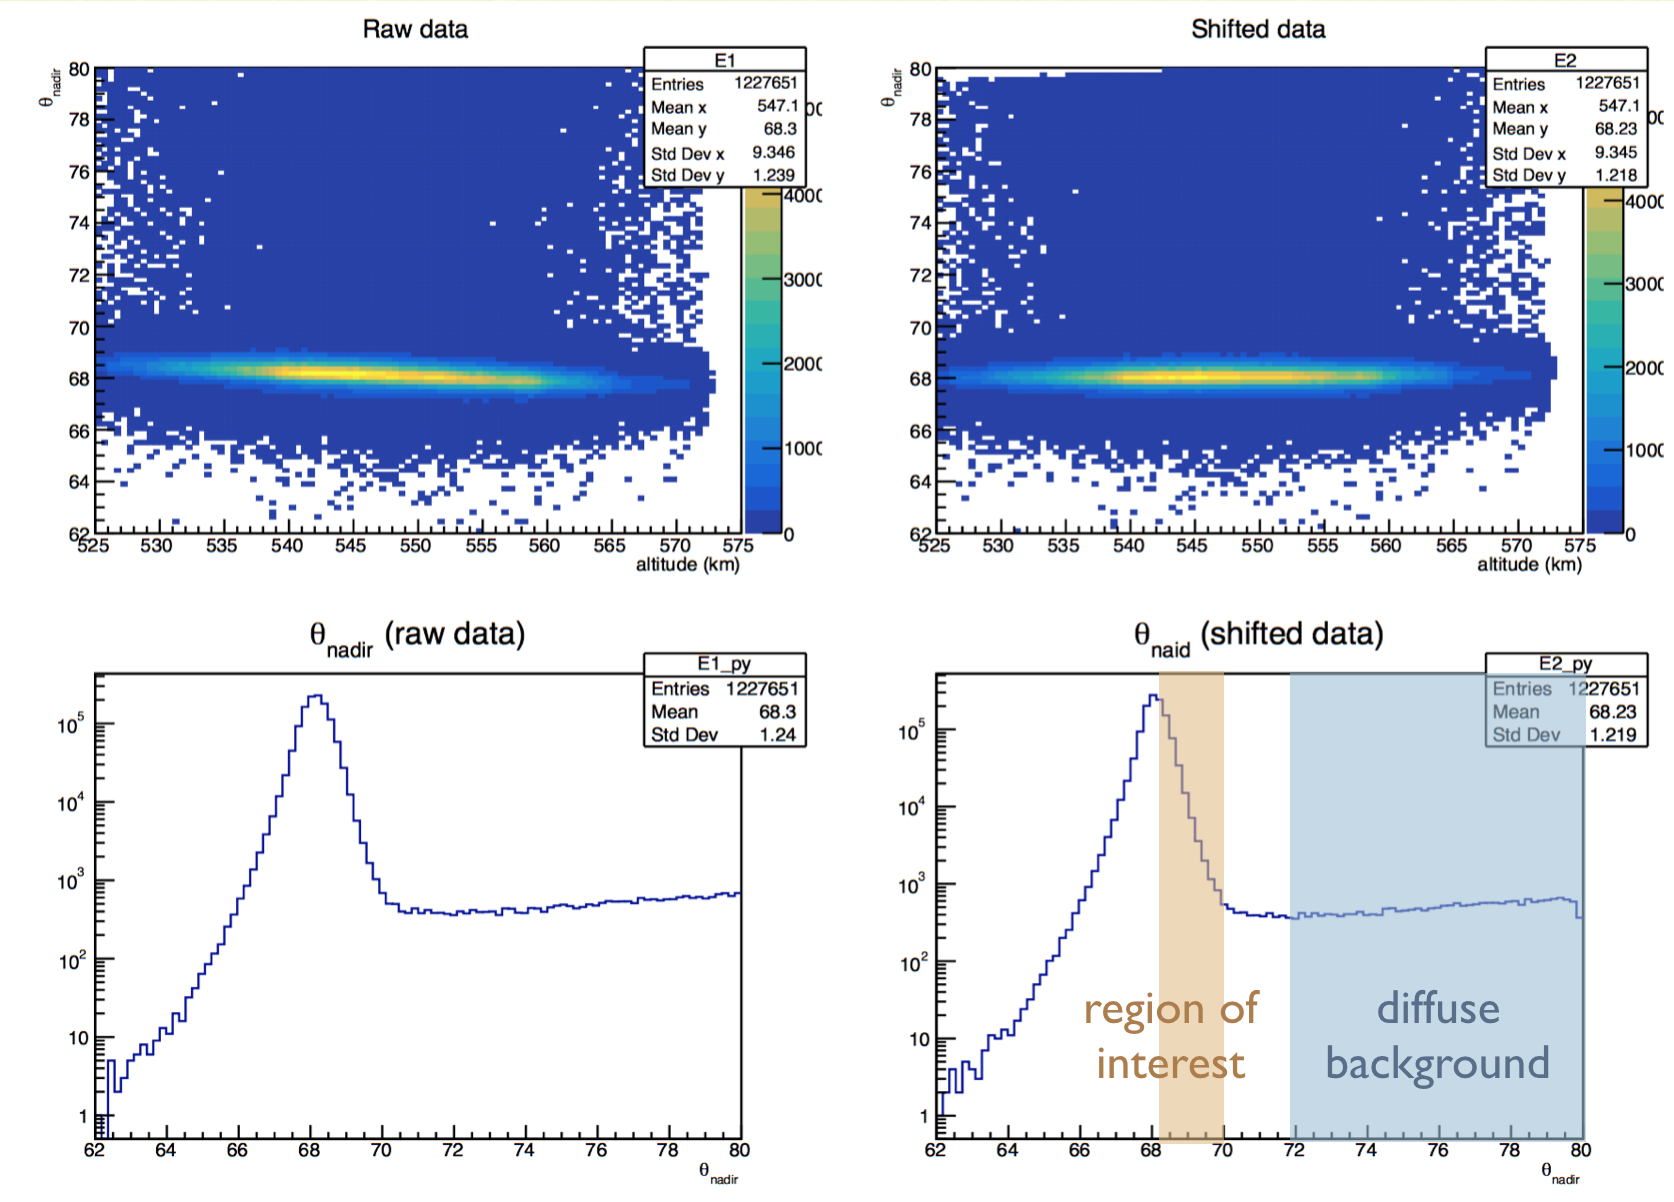
\includegraphics[width=0.8\textwidth]{content/result_and_discussion/figures/LATShifted.png}
    \caption{Distribution of nadir angle before and after altitude correction}
    \label{fig:lat_nadir_shifted}
\end{figure}


The top-left of Figure \ref{fig:lat_nadir_shifted} demonstrates how 
much spacecraft orbiting altitude correlate to the $\theta_\text{NADIR}$
by a 2D heatmap plot of photon intensity. The bottom-left histogram
came from the projection of the previous raw count 2-D histogram which 
has a peak around 68\textdegree. Both bottom and top right histograms
was constructed from exactly the same logic but there is one different 
variable. The shifted nadir angle has been calculated to reduce the 
effect from the spacecraft and the region of interest has been highlighed 
as orange for calculating as the limb spectrum and the blue zone is 
a diffusive background to be used in the background subtraction.

The brightness of Earth's limb is much brighter than the 
diffusive background on the map. The region of interest and 
the background intensity has a huge difference in approximately
an order or magnitude.


\section{$\gamma$-ray spectrum measurement}

According to the definition from Equation \ref{eq:def_flux}, 
the first step is the construction of the count map of the Earth's 
centered coordinates. Regardless of the photon energy, a week of the 
accumulated photon has been plotted in the Figure \ref{fig:sample_photon_dist} to visualize 
the raw count of the sample data on the count map.

\begin{figure}[h!]
    \centering
        \subfloat[
            Photon count map
        ]{
            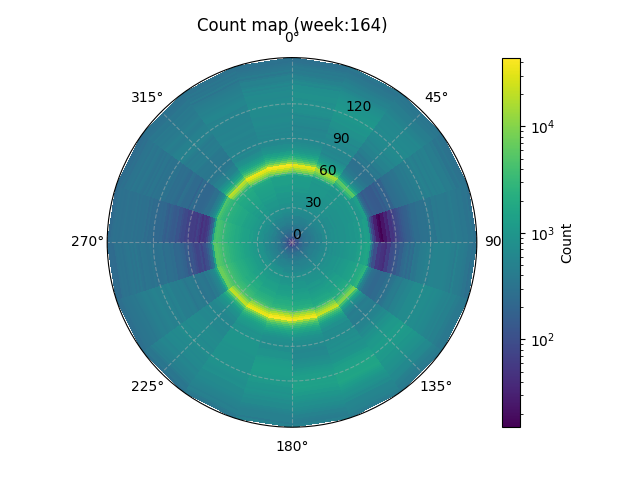
\includegraphics[width=0.48\textwidth]{content/result_and_discussion/figures/cntmap_polar.png}
        }
        \hfill
         \subfloat[
            Photon distribution along the nadir angle
         ]{
            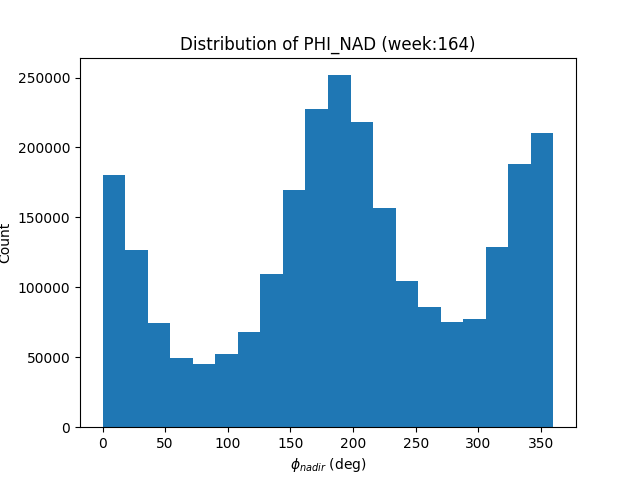
\includegraphics[width=0.48\textwidth]{content/result_and_discussion/figures/phi_nad_dist.png}
        }
        \caption{An example distribution of $\gamma$-ray from a single week}
       \label{fig:sample_photon_dist}
\end{figure}

The limb's region could be easily observed in the bright ring above 
a dashed line of 60\textdegree nadir angle. 
Figure \ref{fig:sample_photon_dist} an also shows the brightness of 
the southern and northern hemispheres. Further investigating of the 
East-West effects could be illustrated by projecting the 2-D histogram 
into 1-D histogram of the nadir angle as in Figure \ref{fig:sample_photon_dist}b.
Nevertheless, the explanation of the East-West a rough description
and still incomplete since it does not take the exposure into account yet.

Applying criteria from the data selection such as event class, LAT's incident angle would affect the result from the histogram filling.
In practice, each histogram was constructed for their belonging bin 
of the histogram in the energy domain. Hence, the multiple count map 
will be created for serving their energy ranges as in the
Figure \ref{fig:cntmap_cartesian}.

\begin{figure}[h!]
    \centering
    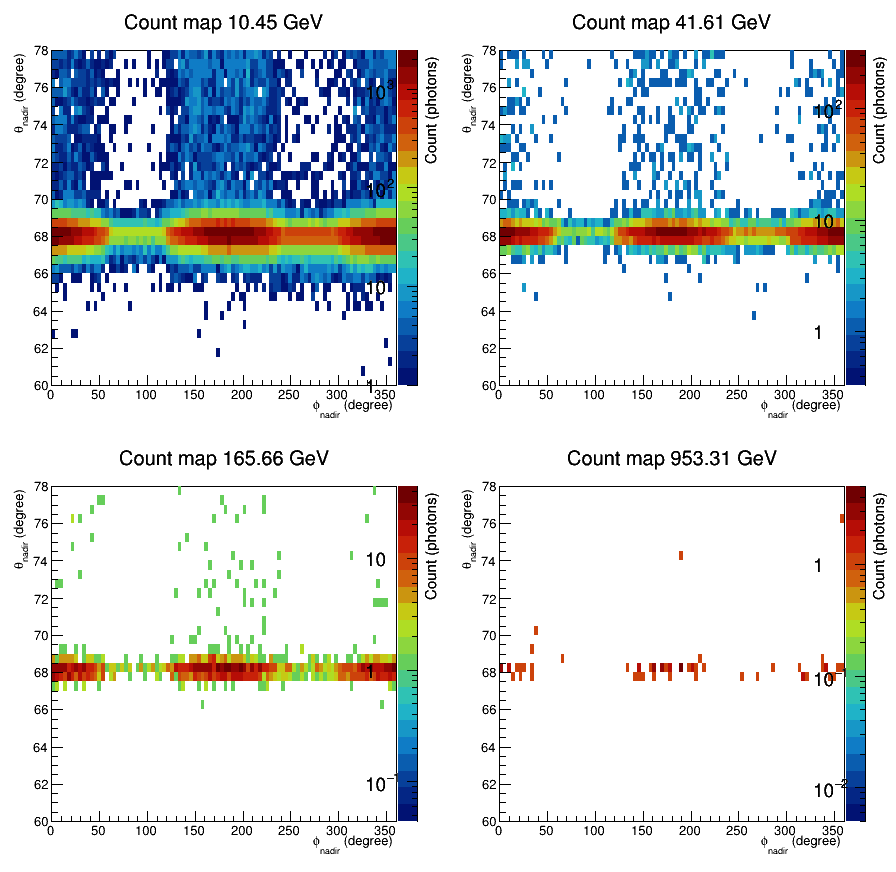
\includegraphics[width=0.8\textwidth]{content/result_and_discussion/figures/cartesian_cntmaps.png}
    \caption{Cartesian plot of the photon histograms (title represent mean of the energy range)}
    \label{fig:cntmap_cartesian}
\end{figure}


\begin{figure}[h!]
    \centering
    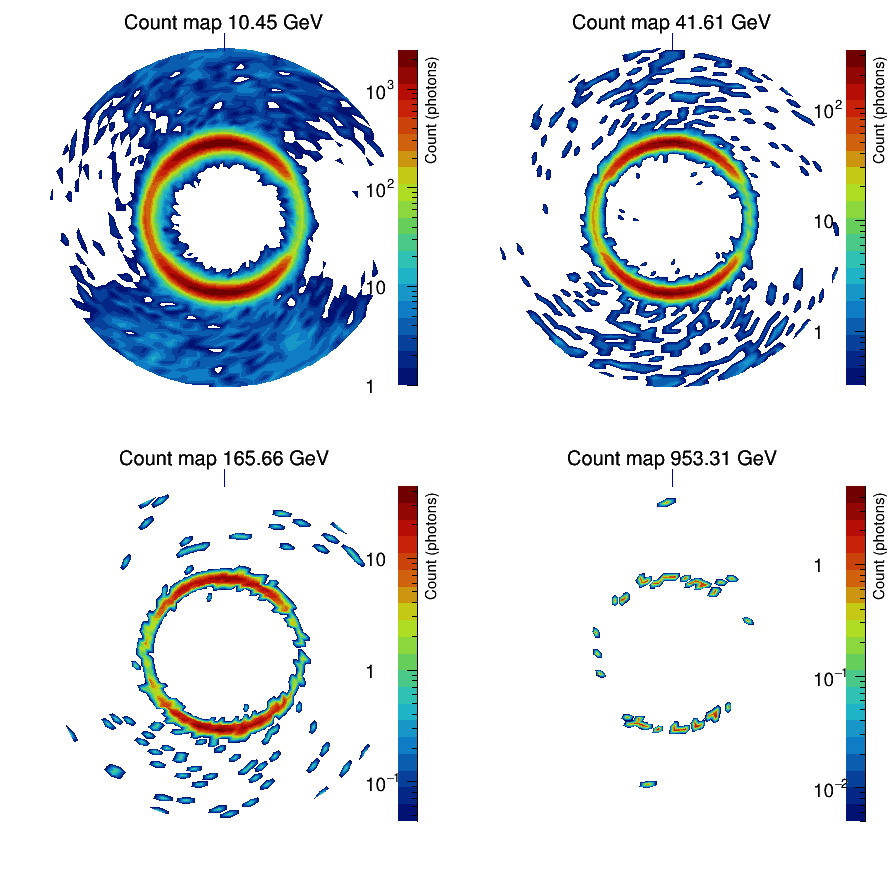
\includegraphics[width=0.8\textwidth]{content/result_and_discussion/figures/polar_cntmaps.png}
    \caption{Polar plot of the photon histograms}
    \label{fig:cntmap_polar}
\end{figure}


However, looking at polar coordinate plotting from the cartesian point of view 
would not be a proper way. Figure \ref{fig:cntmap_polar} is another angle of viewing the same data but in their natural orientations.
Both visualizations show that the Earth's limb region in $\gamma$-ray 
is the shinest band for all interesting energy.
It is also obvious to say that the more energy filtering condition,
the less photon would match the criteria.



The next step is the exposure calculation. The exposure map is computed 
by accumulated exposure time from the LAT's FoV and also takes the 
effectiveness of the detector for correcting an angle dependency.
By the end of the day, a unit from the calculation will be an 
area multiple by the time. The raw cartesian plot is visualized in
Figure \ref{fig:expmap_cartesian} with an attached axis.

\begin{figure}[h!]
    \centering
    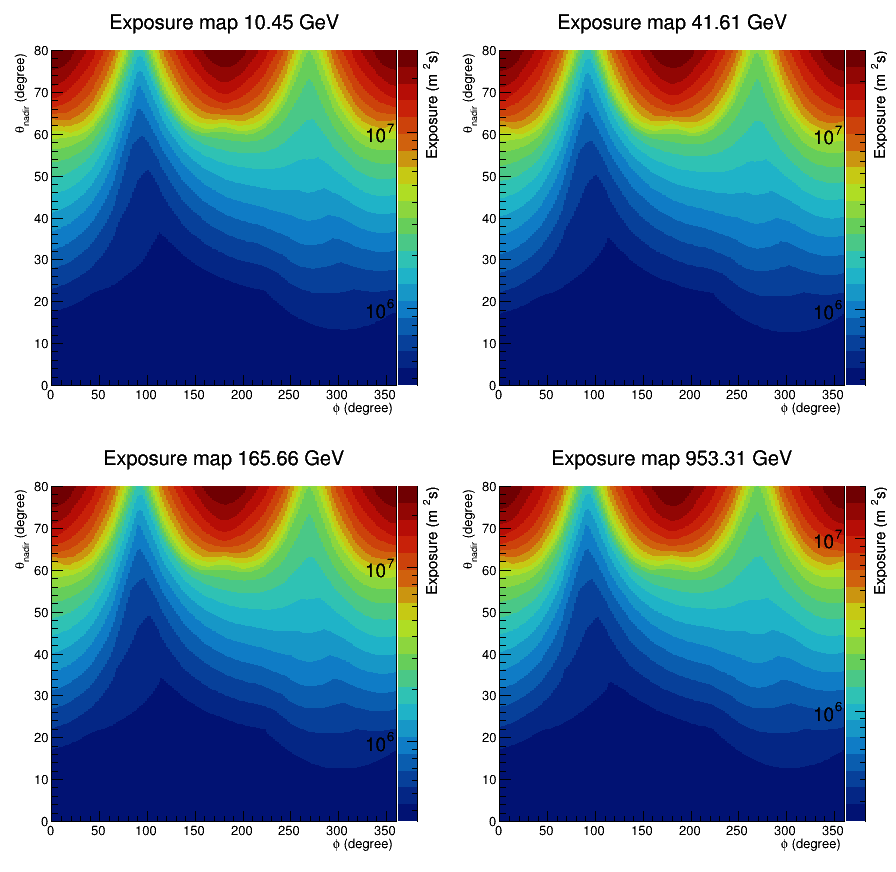
\includegraphics[width=0.8\textwidth]{content/result_and_discussion/figures/cartesian_expmaps.png}
    \caption{Cartesian plot of the exposure histograms}
    \label{fig:expmap_cartesian}
\end{figure}


The heatmaps show that the exposure intensity in the sky is much
higher than the Earth in an order of magnitude because LAT was designed
for seeking flare events in the space rather than looking at Earth.
Regarding a given nadir angle between 60\textdegree to 70 \textdegree,
the spacecraft seems to look at the northern or southern hemisphere 
rather than the eastern and the western side. The color of the 
at 270\textdegree (West) is more intense than 90\textdegree (East)
means that the spacecraft tends to peek in the Westside more
than Eastside. The reason might come from the trajectory of the charged 
particles were bent and produce a $\gamma$-ray which potentially could 
convince LAT to look at them rather than the other side because it 
has a chance to trigger the GBM.
The 2-D histograms in polar coordinates have also been
plotted in Figure \ref{fig:expmap_polar}.

\begin{figure}[h!]
    \centering
    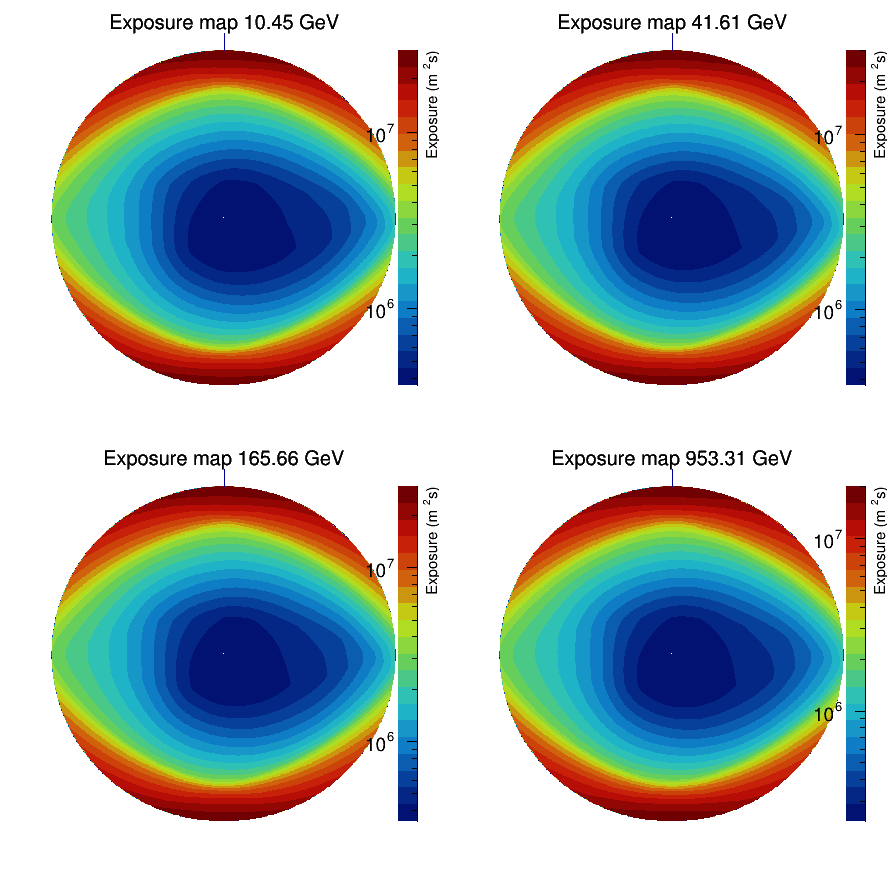
\includegraphics[width=0.8\textwidth]{content/result_and_discussion/figures/polar_expmaps.png}
    \caption{Polar plot of the exposure histograms}
    \label{fig:expmap_polar}
\end{figure}


The last step starts with initiating the new map that was 
defined by the division from the count maps and the exposure maps.
After that, integrating the limb region in the polar coordinates
to get a single scalar value. The scalar is then divided by the 
gap of the energy bin and the solid angle as a unitless quantity.
Repeating a given description for all energy bins in the $\gamma$-ray 
spectrum and subtracts by the background would yield the final 
photon spectrum as in Figure \ref{fig:flxhist}.

\begin{figure}[h!]
    \centering
    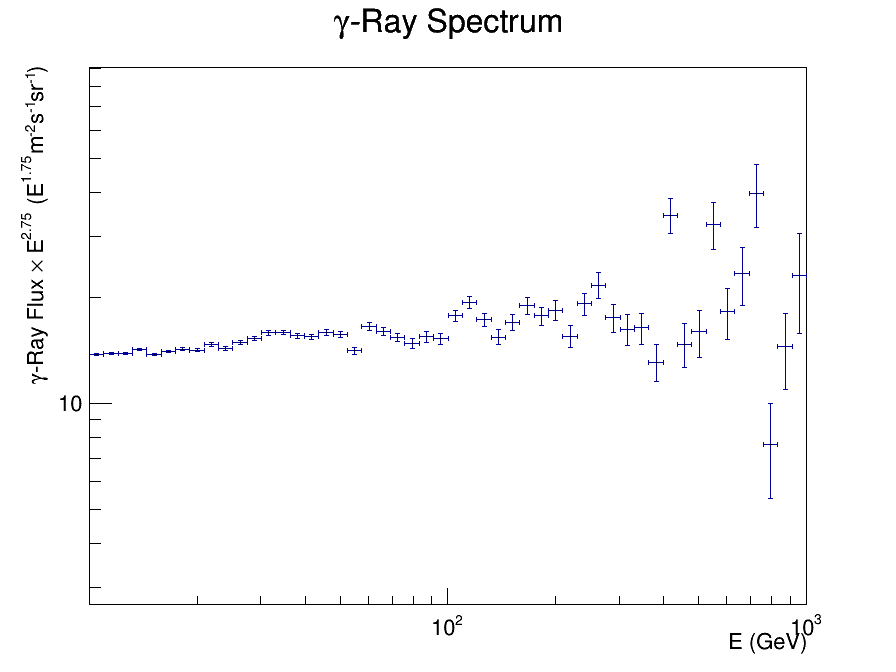
\includegraphics[width=0.7\textwidth]{content/result_and_discussion/figures/flx_hist.png}
    \caption{Measured $\gamma$-ray spectrum}
    \label{fig:flxhist}
\end{figure}

\newpage

In addition, exploring the $\gamma$-ray intensity from the visualization
of the Earth's centered coordinates would be informative aspects
to observe the variation of the photon intensity along the nadir angle as well as the 
East-West effect. The cartesian plotted is in Figure
\ref{fig:flxmap_cartesian} and the polar form as in the Figure 
\ref{fig:flxmap_polar}. Comparing the intensity along the peak of 
theta nadir in the cartesian plot from the East ($\phi$=90\textdegree)
and West ($\phi$=270\textdegree) would reflect that the band of 
the intensity in the west is slightly thicker than in the East and the 
color of the peak center is more a little darker than the other 
side. It means that not only the intensity but also the ring thickness
of the limb region is larger from West to East.


\begin{figure}[h!]
    \centering
    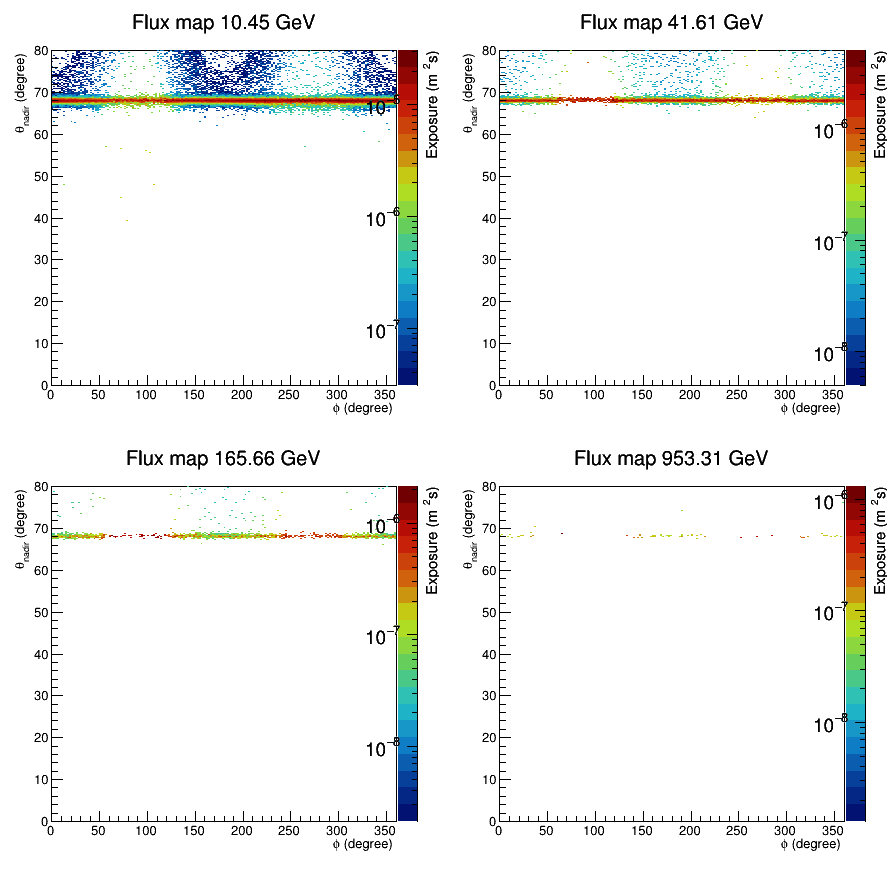
\includegraphics[width=0.8\textwidth]{content/result_and_discussion/figures/cartesian_flxmaps.png}
    \caption{Cartesian plot of the flux histograms}
    \label{fig:flxmap_cartesian}
\end{figure}


\begin{figure}[h!]
    \centering
    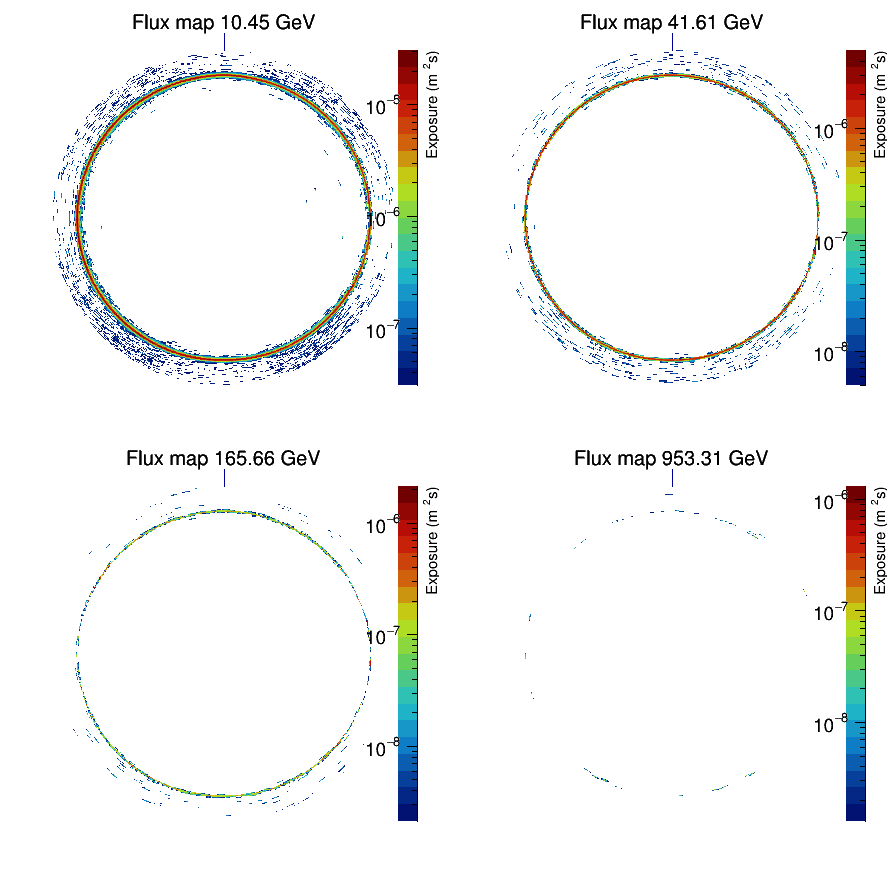
\includegraphics[width=0.8\textwidth]{content/result_and_discussion/figures/polar_flxmaps.png}
    \caption{Polar plot of the flux histograms}
    \label{fig:flxmap_polar}
\end{figure}

\newpage

\section{Best fit result}

The optimized parameters for SPL and BPL models are summarized in 
Table \ref{tb:bestfit}. Best fit $\gamma$-ray from both models are 
visualized in the Figure \ref{fig:fitted_gamma_specgtrum} along
with spectrum from the measurement.

\begin{table}[h!]
    \centering
    \begin{tabular}{l | c | c | c}
      Best fits & $\gamma_1$ & $\gamma_2$ & $E_{\text{Break}}$ (GeV) \\
      \hline \hline
      SPL & 2.70 & - & -  \\
      BPL & 2.86  & 2.63 & 333
    \end{tabular}
    \caption{Optimization results}
    \label{tb:bestfit}
\end{table}

The comparative illustration
also be visualized in the Figure \ref{fig:fitted_cr_proton} with a 
scaled spectra from both models to collate two other direct 
observations of the space-based experiments. It is obvious to see 
the consistency of BPL with the direct measurements in the bellowing 
sub-figure is more corresponding than the SPL model in the top sub-figure
because the breaking point of the BPL does looks more likely to be 
a proper model where the x-axis is the same rigidity scale.

However, a more complex model would perform better than the model 
that has less degree of freedom in practice. Determining the 
statistical significant would be the best way to answer whether 
CR spectrum is naturally described as a BPL indeed.
The significant level could be determined by applying the objective function
to Equation \ref{eq:lrt} for testing one-tail hypothesis-like
from the null hypothesis comparing to an alternative
hypothesis which is the model of breaking of spectral indices
and non-breaking scheme or SPL versus BPL in another word.
The significance is around 1.38$\sigma$ or at 92\%.


\begin{figure}[h!]
    \centering
    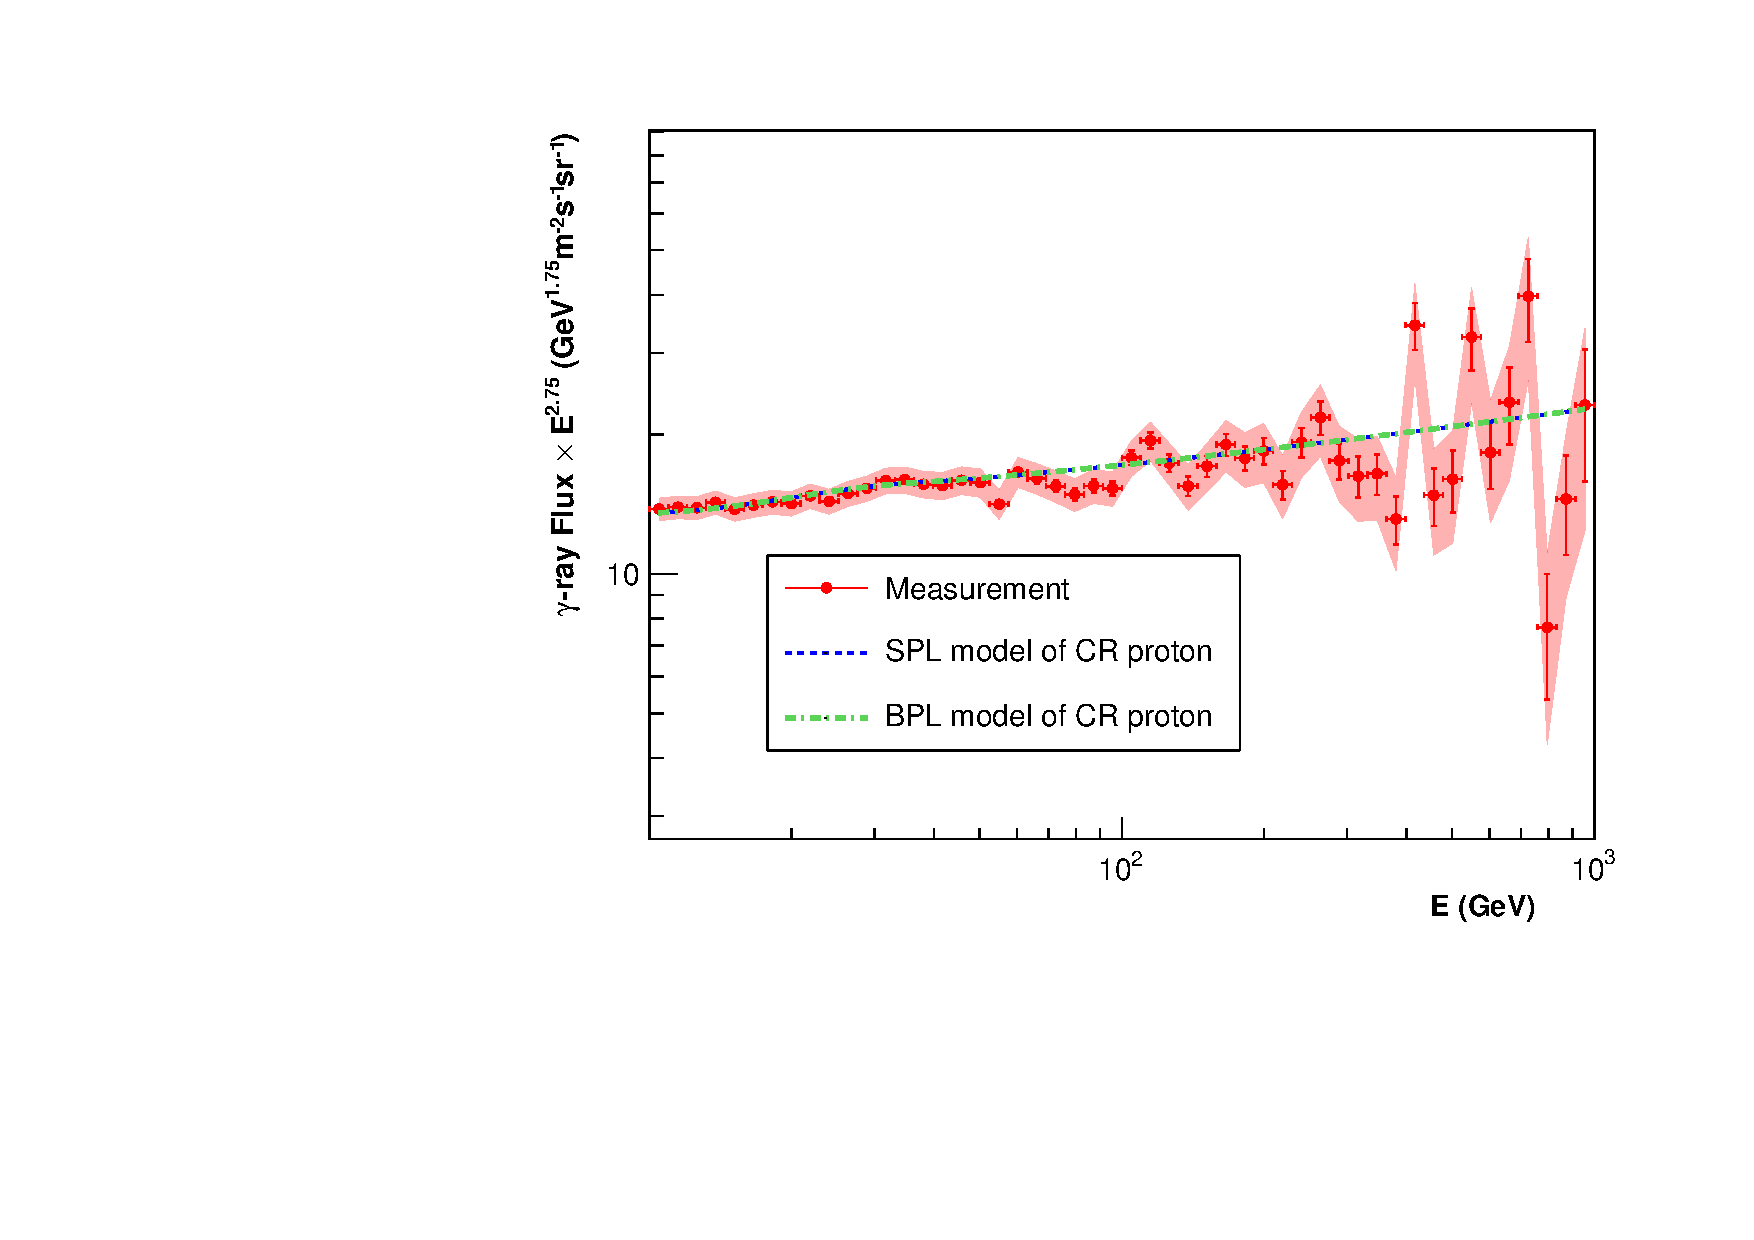
\includegraphics[width=0.8\textwidth]{content/result_and_discussion/figures/fitted_result.pdf}
    \caption{
        The $\gamma$-ray spectra calculated from the SPL (red)
        and BPL (blue) models of CR proton which best fit with the
        measured Earth's $\gamma$-ray spectrum in the thin-target
        regime (red)
    }
    \label{fig:fitted_gamma_specgtrum}
\end{figure}

\newpage 

\begin{figure}[h!]
    \centering
    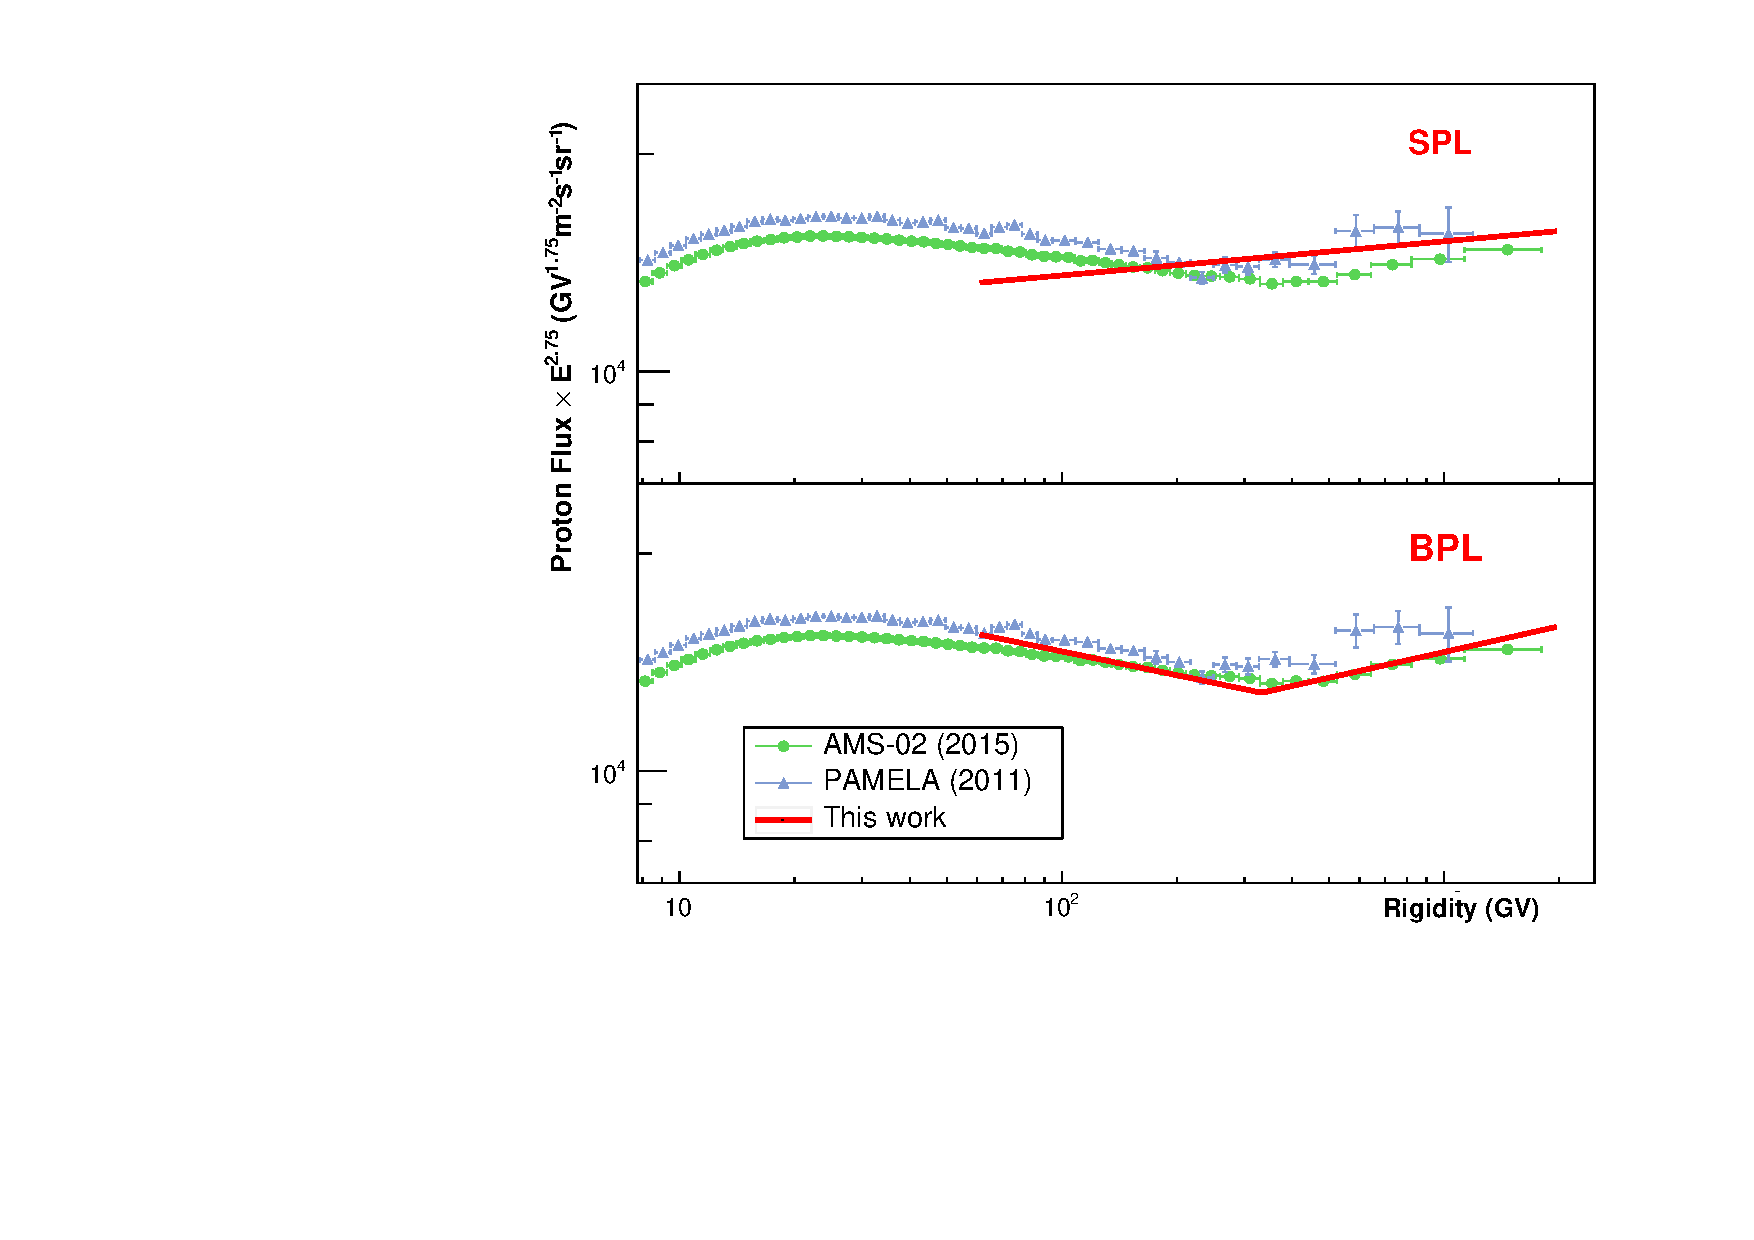
\includegraphics[width=0.9\textwidth]{content/result_and_discussion/figures/ProtonSpectrumModelMeasurement.pdf}
    \caption{
        Best-fit CR proton spectrum from this work (red)
        compared to the measurementsby AMS-02 (blue) and
        PAMELA (green)
    }
    \label{fig:fitted_cr_proton}
\end{figure}

